\section{Results}

\subsection{Datasets}\label{sec:results:data}

%\mdeff{All stuff about data here.
%Ideally same data for all experiments.}
%\todo{Merge and shorten.}
%\todo{$P$ training projections.}

We consider two proteins as ground truths: the $\beta$-galactosidase, a protein with a dihedral (D2) symmetry, and the lambda excision HJ intermediate (HJI), an asymmetric protein.
Their deposited PDB atomic models are 5a1a ~\cite{bartesaghi2015betagal} and 5j0n~\cite{laxmikanthan2016structure}, respectively.
For each atomic model, we generate the ground truth by fitting a 5\AA\ density map in Chimera~\cite{pettersen2004ucsf}.
We thus obtain a volume of size $110\times 155\times 199$ for the $\beta$-galactosidase, and a volume of size $69\times 57\times 75$ for the HJI.

\paragraph{Generating Projections} 
From these ground truths, we generate $5,000$ synthetic projections of size $275\times 275$ and $116\times 116$, respectively, using the ASTRA projector~\cite{van2015astra}.
The projection orientations are sampled from a uniform distribution of Euler angles on half of the $\SO(3)$ space, which suffices to generate all the possible projections of a volume.
Initially, for the sake of simplicity, the projections are kept unblurred and noiseless, later we add noise and translation. Examples of these projections can be seen in Figure \ref{fig:different-projections}.

\begin{figure}
    \centering
    \begin{subfigure}[b]{0.3\textwidth}
        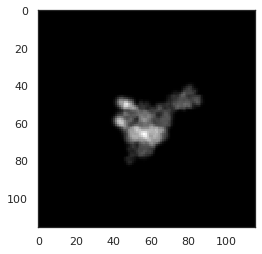
\includegraphics[height=4cm]{images/5j0n_noise0.png}
        \caption{}
    \end{subfigure}
    \hfill
    \begin{subfigure}[b]{0.3\textwidth}
    \centering
        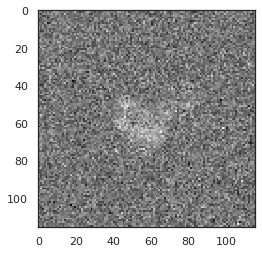
\includegraphics[height=4cm]{images/5j0n_noise16.png}
        \caption{}
    \end{subfigure}
    \hfill
    \begin{subfigure}[b]{0.3\textwidth}
    \centering
        \includegraphics[height=4cm]{images/5j0n_translation.png}
        \caption{}
    \end{subfigure}
    \caption{Different projection types:
    \textbf{(a)} Projections without noise nor translation
    \textbf{(b)} Projections with white noise with variance 16
    \textbf{(c)} Projections with translation.}
    \label{fig:different-projections}
\end{figure}



\paragraph{Generating a Proper Training Dataset for the Distance Estimation}
We use supervised learning, thus input-output pairs. 
The input are two images and the output is their quaternion distance calculated from the ground truth orientations. 
For neural network training, dataset is split into a distinct training, validation, and testing set, see Table \ref{table:dataset}, to ensure that the results can generalize to unseen projections.


\begin{table}[h!]
\centering
\begin{tabular}{||c | c c c||} 
 \hline
 Dataset & Number of images (\%) & Maximum number of projection pairs & Number of projection pairs used\\ [0.5ex] 
 \hline\hline
Train set & 2512 (50\%) & 6,312,656 & 63,126 (1\%)\\ 
Validation set & 1650 (33\%) & 2,722,500 & 27,225 (1\%)\\ 
Test set & 837 (17\%) & 701,406 & randomly sampled per batch \\ [1ex] 
 \hline
\end{tabular}
\caption{Training, validation, and test dataset sizes}
\label{table:dataset}
\end{table}


\paragraph{Dataset for the Orientation Recovery}
The training for the orientation recovery was done in a stochastic setting, where the loss function varies over the batches.
The dataset used in this part is test set from Table \ref{table:dataset}. This way, the orientation recovery will be performed on the projections unseen by the previously trained network.


\subsection{Evaluation}\label{sec:results:evaluation}

\mdeff{Story: need to know how good we did (without reconstructing the protein).
As orientations are up to a global rotation/mirror on $\SO(3) / \mathbb{S}^3$, best align recovered and true orientations before computing the mean recovery error.}

\todo{Introduce the mean recovery error as a good and intuitive performance metric.}
\todo{Figure that shows a typical convergence and mean orientation recovery error before and after alignment. We'll subsequently only report $E$ (the error after alignment).}

Before discussing the results, we remark that one cannot really quantify the performance of~\eqnref{orientation-recovery} through its loss.
Unfortunately, it is also not appropriate to directly compute the error between the recovered orientations $\big\{\widehat{q}_p\big\}_{p=1}^P$ and the true ones $\big\{q_p\big\}_{p=1}^P$.
The reason is that the recovery of orientation through~\eqnref{orientation-recovery} is up to a global rotation, \textit{i.e.}, any global rotation of the set of recovered orientations is as valid as any other.
This is not a problem for the ultimate application of our scheme, but it complicates the quantitative evaluation of its performance in synthetic experiments.
We circumvent this problem by aligning the true and recovered orientation sets \textit{i.e.} objective is to minimize the distance difference between these two sets.

\begin{figure}
    \centering
    \begin{subfigure}[b]{0.45\textwidth}
        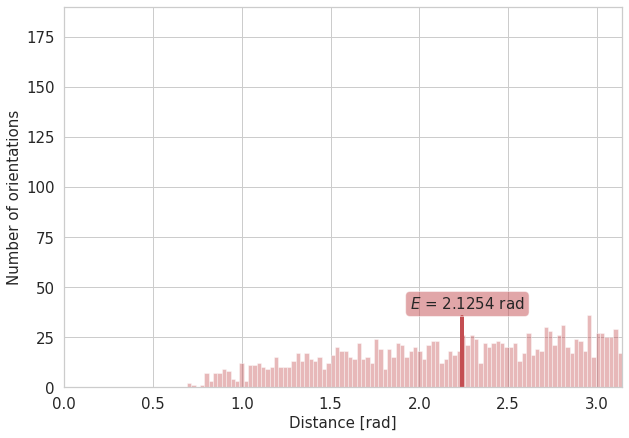
\includegraphics[height=5.7cm]{images/5j0n_noise0_angle_alignment_before.png}
        \caption{Before orientation alignment}
    \end{subfigure}
    \hfill
    \begin{subfigure}[b]{0.5\textwidth}
    \centering
        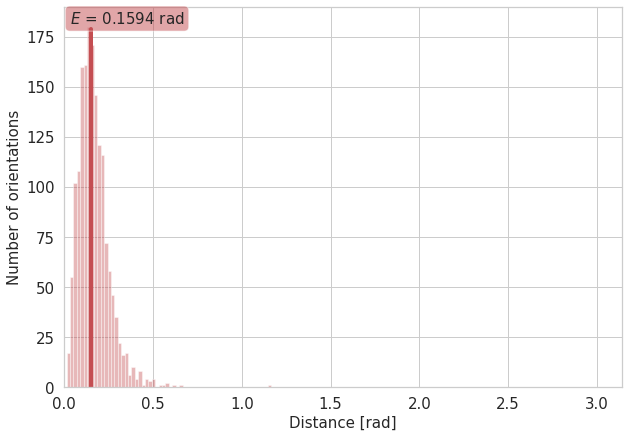
\includegraphics[height=5.7cm]{images/5j0n_noise0_angle_alignment_after.png}
        \caption{After orientation alignment}
    \end{subfigure}
    \caption{
        Mean orientation recovery error of the asymmetric protein (5j0n).
}
    \label{fig:angle-alignment-5j0n-noise0}
\end{figure}

\begin{figure}
    \centering
    \begin{subfigure}[b]{0.45\textwidth}
        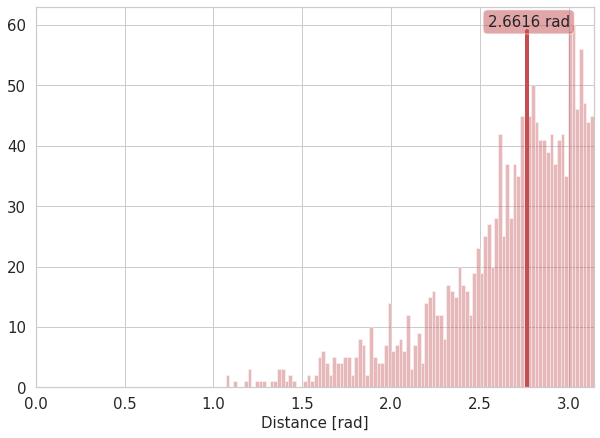
\includegraphics[height=5.7cm]{images/5j0n_noise16_angle_alignment_before.png}
        \caption{Before orientation alignment}
    \end{subfigure}
    \hfill
    \begin{subfigure}[b]{0.5\textwidth}
    \centering
        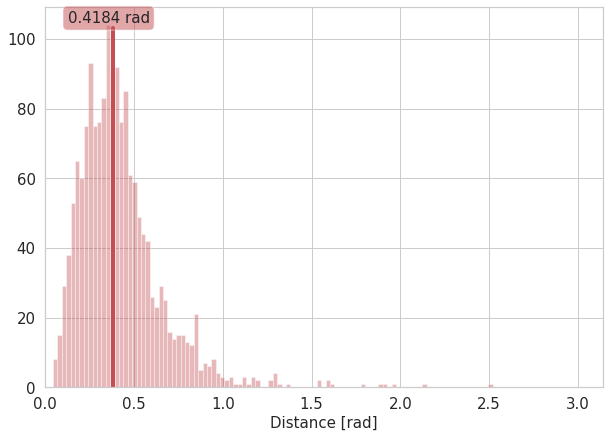
\includegraphics[height=5.7cm]{images/5j0n_noise16_angle_alignment_after.png}
        \caption{After orientation alignment}
    \end{subfigure}
    \caption{
        Mean orientation recovery error of the asymmetric protein (5j0n) with white noise (variance 16).
}
    \label{fig:angle-alignment-5j0n-noise16}
\end{figure}

The goal of the alignment is to find the \textit{mean orientation recovery error} using gradient descent methods. The variable of the optimization problem is the orthogonal matrix (with determinant $\pm1$)   $\mathbf{T}\in\Or(4)$
\begin{equation}
    E = \min_{\T \in \Or(4)} \frac{1}{P_{test}} \sum_{i} \big| d_q\left(q_i,\mathbf{T}\hat{q_i}\right)\big|^2,
    \label{eqn:orientation-recovery-error}
\end{equation}
where $\Or(4) = \{\T | \det(\T) = \pm 1\}$ is the group of $4 \times 4$ orthogonal matrices that represent 4D rotations and reflections, and $P_{test}$ is the number of projections in test set.
In practice, the sum is again sampled and \eqnref{orientation-recovery-error} is separately minimized using gradient descent method with FTRL optimizer \cite{TODO} for $\det(\T) = 1$ and $\det(\T) = -1$ because $\Or(4)$ is disconnected.
%Note the similarity with~\eqnref{metric-learning} and~\eqnref{orientation-recovery}.
% \mdeff{We do normalize by the number of pairs right?}

The mean orientation recovery error for asymmetric protein 5j0n without noise in the projection can be seen in Figure \ref{fig:angle-alignment-5j0n-noise0}. Experimental setting parameters are: 3 runs per reflection (total number of runs is 6), 300 steps, batch size 256, FTRL optimizer with learning rate 2.0 and learning rate power -2.0. The smallest error achieved is 0.1594 rad.

The mean orientation recovery error for asymmetric protein 5j0n with noisy projections (white noise with variance 16) can be seen in Figure \ref{fig:angle-alignment-5j0n-noise16}. Experimental setting parameters are: 3 runs per reflection (total number of runs is 6), 300 steps, batch size 256, FTRL optimizer with learning rate 2.0 and learning rate power -2.0. The smallest error achieved is 0.4184 rad.



\subsection{Orientation recovery}\label{sec:results:orientation-recovery}

\mdeff{Story: good distance estimation = good orientation recovery.}
\mdeff{(Nothing to write here.)}

%\subsubsection{Feasibility Check: Recovery from the Exact Relative Distances}
\subsubsection{Recovery from exact distances}\label{sec:results:orientation-recovery:exact}

\begin{figure}[b]
    \centering
    \begin{subfigure}[b]{0.45\textwidth}
        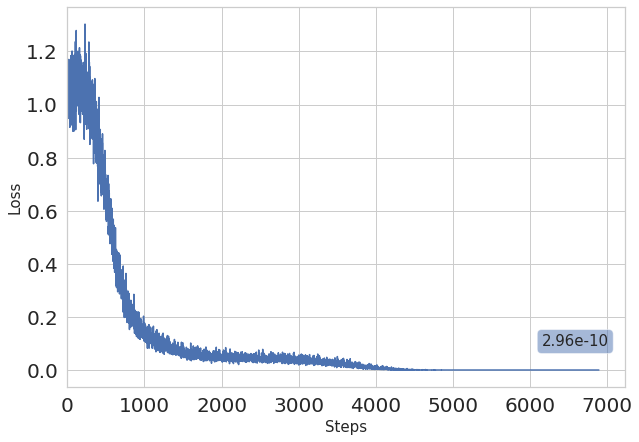
\includegraphics[height=5.5cm]{images/5j0n_perfect_angle_recovery.png}
        \caption{Asymmetric protein (5j0n)}
    \end{subfigure}
    \hfill
    \begin{subfigure}[b]{0.5\textwidth}
    \centering
        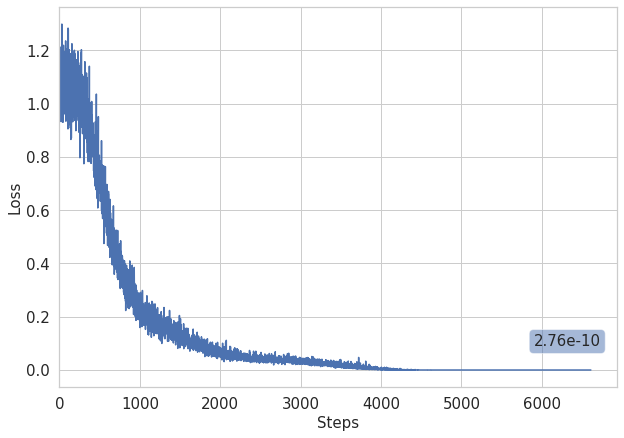
\includegraphics[height=5.5cm]{images/5a1a_perfect_angle_recovery.png}
        \caption{Symmetric protein (5a1a)}
    \end{subfigure}
    \caption{ Orientation recovery loss with the true distances, $d_p(\p_i, \p_j) = d_q(q_i, q_j)$.}
    \label{fig:orientation-recovery-loss}
\end{figure}

\begin{figure}[!]
    \centering
    \begin{subfigure}[b]{0.45\textwidth}
        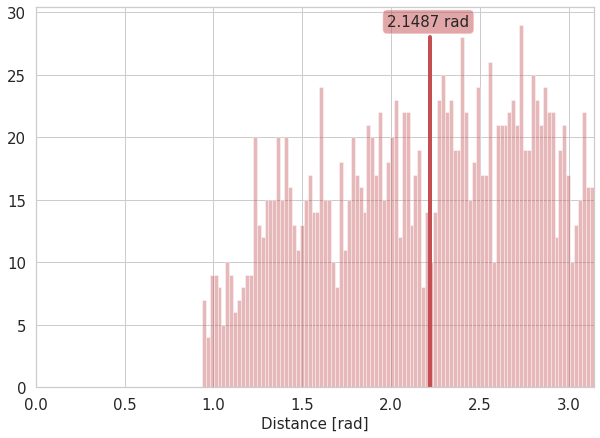
\includegraphics[height=5.5cm]{images/5j0n_perfect_angle_ralignment_before.png}
        \caption{Before the alignment}
    \end{subfigure}
    \hfill
    \begin{subfigure}[b]{0.5\textwidth}
    \centering
        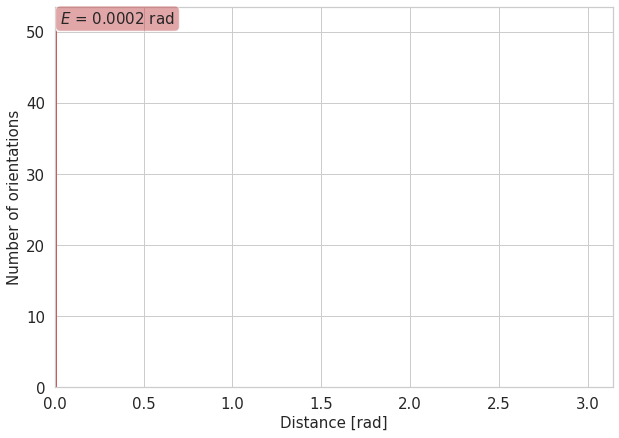
\includegraphics[height=5.5cm]{images/5j0n_perfect_angle_ralignment_after.png}
        \caption{After the alignment}
    \end{subfigure}
    \caption{ Example of perfect alignment: mean orientation error of true distances for asymmetric protein (5j0n) before and after the alignment.}
    \label{fig:angle-alignment-perfect}
\end{figure}

\mdeff{Story: works perfectly despite no convexity guarantee and sampling.}
\mdeff{I made it concise but precise.
Let's do that for all!}

To verify that (i) the lack of a convexity guarantee for \eqnref{orientation-recovery} and (ii) the severe sampling of the sum are non-issues in practice, we attempt orientation recovery under exact distance estimation $d_p(\p_i, \p_j) = d_q(q_i, q_j)$.
From $P=5000$ projections taken from one side of the asymmetric protein (5j0n), we sample $5000$ out of $P^2 = \num{25e6}$ pairs and minimize \eqnref{orientation-recovery} with Adam~\cite{kingma2014adam}, a variant of SGD, for $\num{30e3}$ steps ($\sim 1$ hour) with a learning rate of $0.1$.
Orientations are perfectly recovered.
\figref{minim-loss-perfect-distances} shows the convergence of~\eqnref{orientation-recovery} to zero.

\begin{figure}
    \centering
    \begin{subfigure}[b]{0.45\textwidth}
        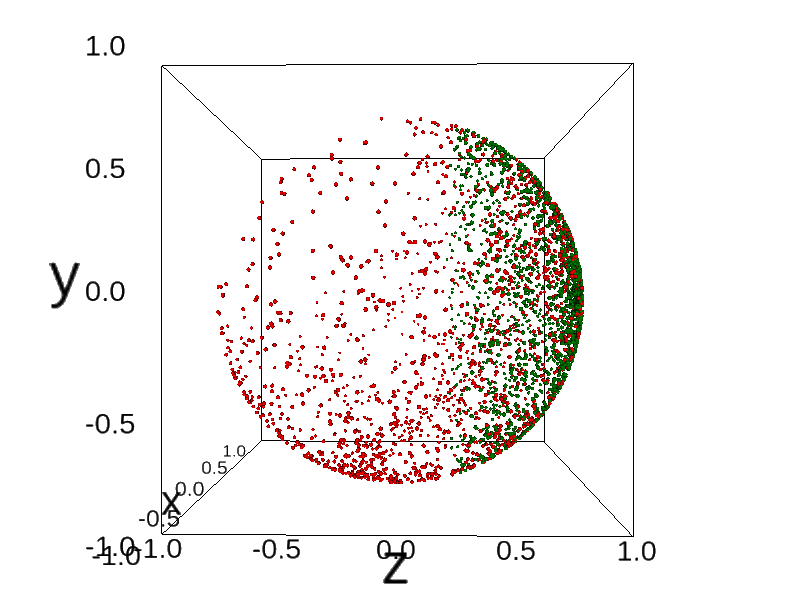
\includegraphics[height=6cm]{images/coverage_alignment_before.png}
        \caption{Before the alignment}
    \end{subfigure}
    \hfill
    \begin{subfigure}[b]{0.50\textwidth}
    \centering
        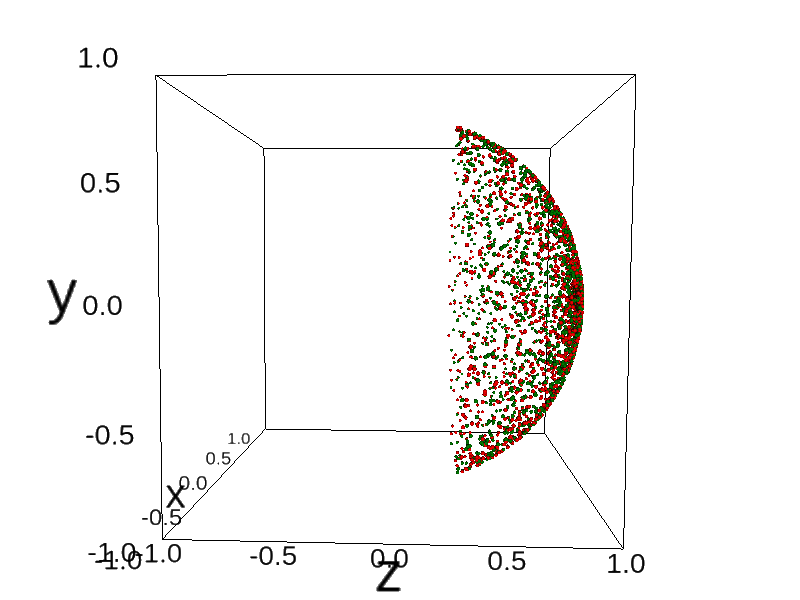
\includegraphics[height=6cm]{images/coverage_alignment_after.png}
        \caption{After the alignment}
    \end{subfigure}
    \caption{
        Orientation coverage of $\mathbb{S}^2 \subset \SO(3)$ after recovery. Green are ground truth orientations and red are estimated orientations.
        % orientations projected on S²
}
    \label{fig:minim-loss-perfect-distances}
\end{figure}

%\subsubsection{Robustness of Recovery to Additive Errors on the Relative Distances}
\subsubsection{Sensitivity to distance estimation error}\label{sec:results:orientation-recovery:sensitivity}

\mdeff{Story: (i) orientation recovery error is strongly linked to distance estimation error, (ii) recovery loss is a good proxy of mean recovery error.}

We now go one step further and evaluate the behaviour of~\eqnref{orientation-recovery} when the true relative distances are corrupted by  additive Gaussian noise.

The experimental conditions are the same than in the previous section, except that we add an error with increasing variance on the relative distances prior to the minimization.
The results are presented in \figref{perfect-with-noise-ar-aa} (red curve).


\begin{figure}
    \centering
    \begin{subfigure}[b]{0.48\textwidth}
        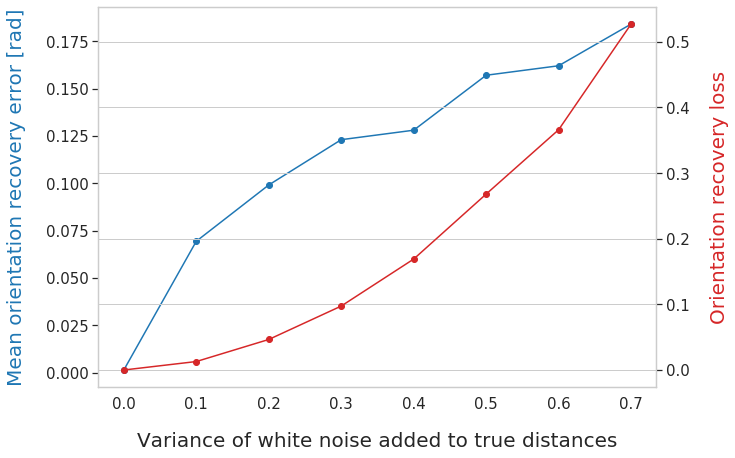
\includegraphics[height=5.15cm]{images/5j0n_perfect_noisy_ar_aa.png}
        \caption{Asymmetric protein (5j0n)}
    \end{subfigure}
    \hfill
    \begin{subfigure}[b]{0.50\textwidth}
    \centering
        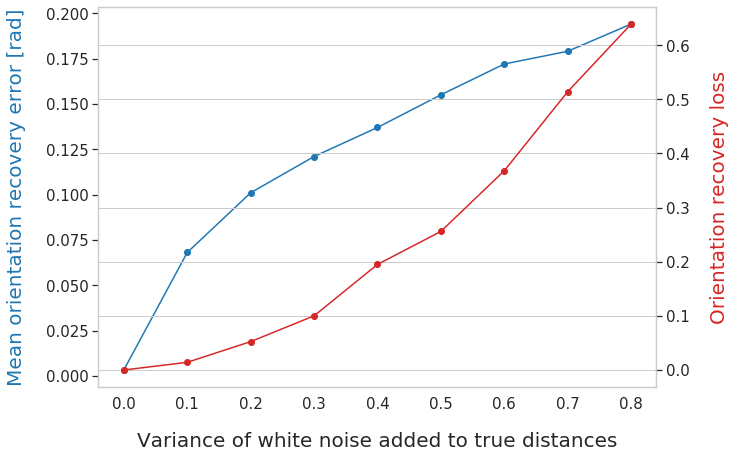
\includegraphics[height=5.15cm]{images/5a1a_perfect_noisy_ar_aa.png}
        \caption{Symmetric protein (5a1a)}
    \end{subfigure}
    \caption{
        The mean orientation recovery error \todo{(eq)} is a monotonic function of the distance estimation error.
        Better distance estimation leads to better orientation recovery.
        Moreover, the recovery loss \todo{(eq)} is a good proxy for the recovery error, allowing us to assess recovery performance without ground-truth orientations.
}
    \label{fig:perfect-with-noise-ar-aa}
\end{figure}

For all variances, the distance after alignment is reported in \figref{perfect-with-noise-ar-aa} (blue curve).

These results demonstrate that the performance of the minimization scheme~\eqnref{orientation-recovery} linearly depends on the quality of the relative distances, which advocates for a proper and extensive training of the SiameseNN in the next stages of development.
Another interesting output of \figref{perfect-with-noise-ar-aa} is that it indicates that the error of the orientation recovery behaves as a monotonic function of its loss.
Hence, it suggests that the loss can be used as a good indicator of its performance, which has obvious practical implications for our future works on real data.

\subsection{Distance estimation}\label{sec:results:distance-estimation}
%\subsection{Estimating Relative Orientations from Projections}
%\subsection{Relative orientation estimation}

\mdeff{Story: $d_p$ good estimator of $d_q$.
SiameseNN better than l2, but still plateaus.
Robust to projection noise.}

\mdeff{Could we quickly try translations? Should be no problem for Siamese.}



\subsubsection{Euclidean distance}\label{sec:results:distance-estimation:euclidean}

\mdeff{Story: simplest baseline estimator, $d_{pe}$ somewhat estimates $d_q$, quickly plateaus (even in the simplest noiseless and centered case).
Note the difference between symmetric and asymmetric proteins.}

As a baseline, we first evaluate the suitability of the Euclidean distance as a projection distance $d_b$ to predict $d_q$.
For the two aforementioned datasets, we randomly select $1,000$ pairs of projections.
For each pair, we compute the Euclidean distance between the projections $d_b(\mathbf{b}^i,\mathbf{b}^j)=\lVert\mathbf{b}^i-\mathbf{b}^j\rVert_2$ and their relative orientation $d_p(q_i,q_j)$ through~\eqnref{distance:orientations}.
We then report the $(d_q,d_b)$ relationship for all pairs in \figref{euclidean-not-robust}, for both the asymmetric protein (left) and the symmetric one (right).

\begin{figure}
    \centering
    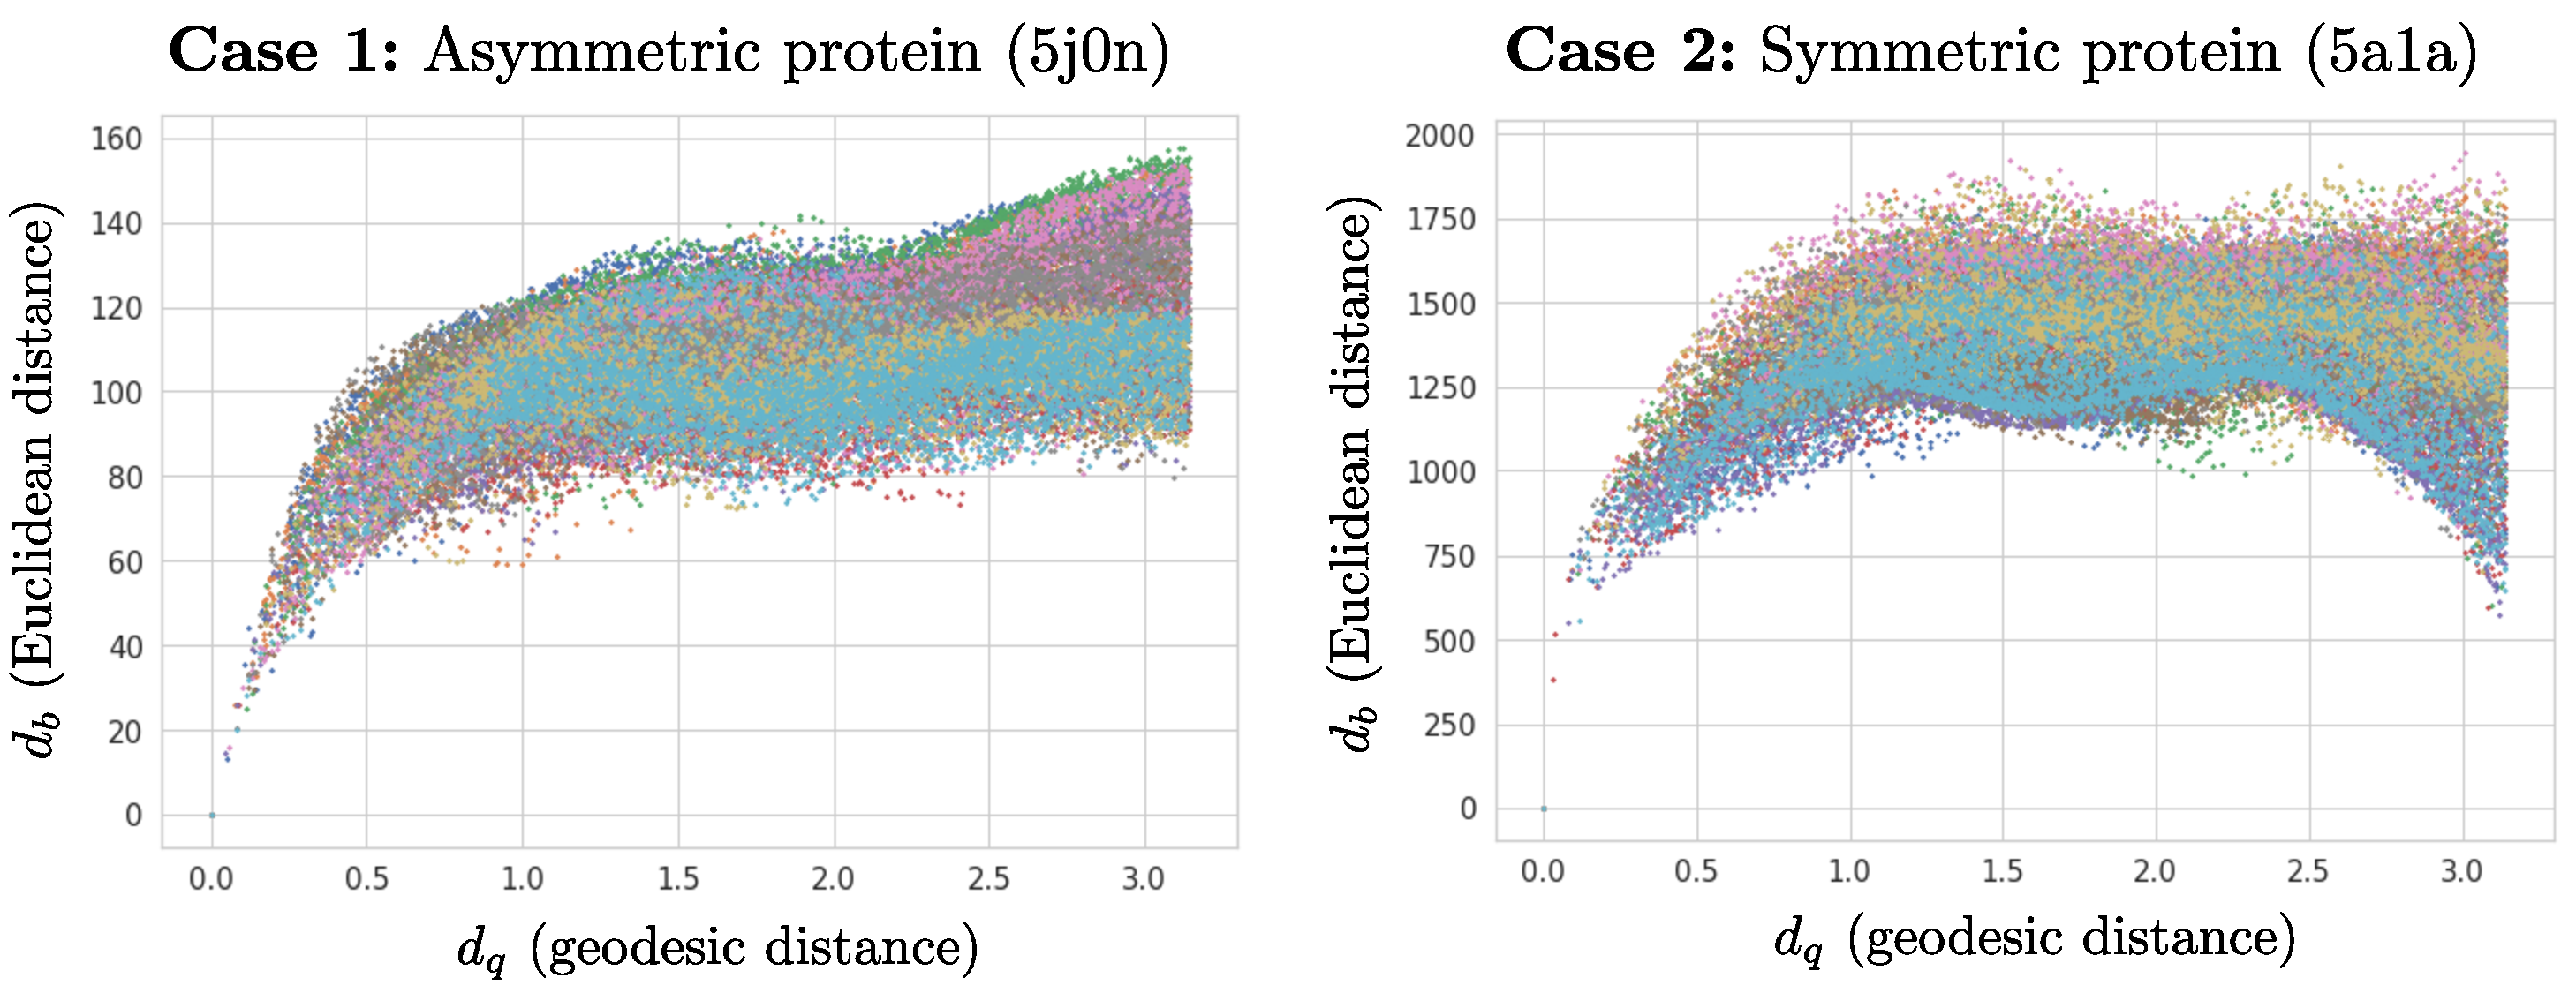
\includegraphics[width=\textwidth]{EuclideanDistance_NonRobust}
    \caption{
        Plotting the Euclidean distance between two projections versus their actual relative orientation (measured by the geodesic distance) for \textbf{(left)} the asymmetric protein (5j0n) dataset, and \textbf{(right)} the symmetric protein (5a1a) dataset. The color corresponds to projection pairs that share the first projection \textit{i.e.} distance between one projection with all other projections.
    }
    \label{fig:euclidean-not-robust}
\end{figure}

Two principal observations can be made from this experiment.
First, as suspected, the Euclidean distance between projections fails to be a consistent predictor of their relative orientation distance, even in the simple imaging conditions considered here (no noise and no effect of the PSF).
In particular, the larger the relative distance $d_q$, the poorer the predictive ability of the Euclidean distance as $d_b$.
The other interesting observation is that the intrinsic symmetry of the $\beta$-galactosidase protein (5a1a) appears in its $(d_q,d_b)$ plot.

\subsubsection{Learned distance}\label{sec:results:distance-estimation:learned}

\begin{figure}
    \centering
    \includegraphics[height=5.5cm]{images/de_architecture.png}
    \caption{Distance estimation network architecture.}
    \label{fig:de-architecture}
\end{figure}

\mdeff{Story: learned distance $d_{ps}$ estimates $d_q$ with some variance but still underestimates larger distances.
Again symmetric vs asymmetric.}

\begin{figure}
    \centering
    \begin{subfigure}[t]{0.45\textwidth}
        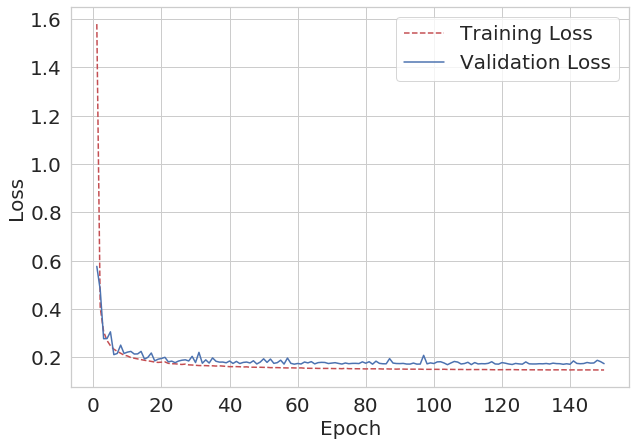
\includegraphics[height=5.5cm]{images/de_5j0n.png}
        \caption{Asymmetric protein (5j0n)}
        \label{fig:losses-siamese-assym}
    \end{subfigure} \quad \quad
    \begin{subfigure}[t]{0.5\textwidth}
        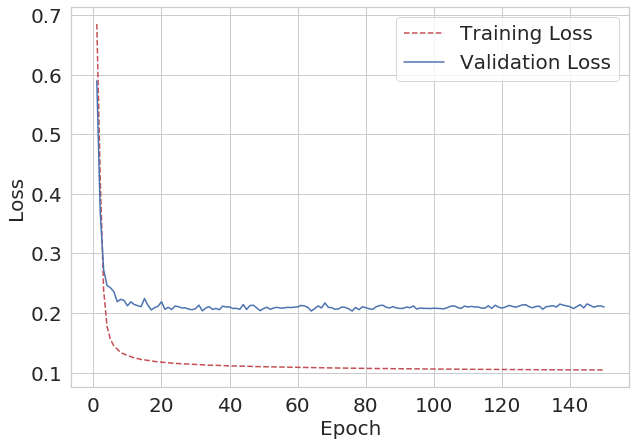
\includegraphics[height=5.5cm]{images/de_5a1a.png}
        \caption{Symmetric protein (5a1a)}
        \label{fig:losses-siamese-sym}
    \end{subfigure}
    \caption{Distance estimation losses on the train and validation datasets.}
    \label{fig:losses-siamese}
\end{figure}

\begin{figure}
    \centering
    \begin{subfigure}[b]{0.45\textwidth}
        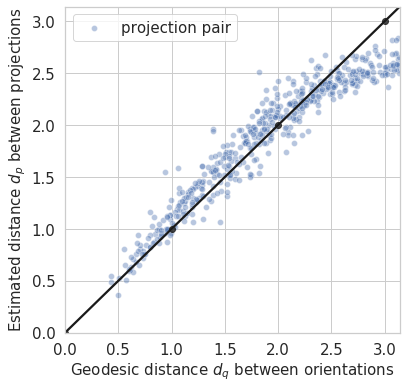
\includegraphics[height=6cm]{images/dPdQ_5j0n.png}
        \caption{Asymmetric protein (5j0n) on test dataset}
    \end{subfigure}
    \hfill
    \begin{subfigure}[b]{0.50\textwidth}
    \centering
        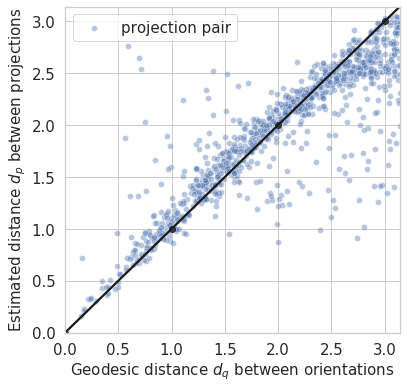
\includegraphics[height=6cm]{images/dPdQ_5a1a.png}
        \caption{Symmetric protein (5a1a) on test dataset}
    \end{subfigure}
    \caption{Relationship between orientations' distance $d_q$ and estimated distance $d_p$.}
    \label{fig:minim-loss-perfect-distances}
\end{figure}

We present here a preliminary evaluation of the ability of SiameseNNs to learn a projection distance $\widehat{d}_b$ that correctly approximates the orientation distance $d_q$.

SiameseNNs come with a variety of more or less powerful architectures.
At the current stage of development, we work with a simple one.
Our SiameseNN is composed of two convolutional neural networks (CNNs) with shared weights.
Their output features vectors are compared through an Eulidean distance, \textit{i.e.}, $F(\mathbf{x},\mathbf{y})=\lVert \mathbf{x}-\mathbf{y}\rVert_2$ in \figref{schematic:distance-learning}.
\todo{The detailed architecture of the SiameseNN is given in figref.}
\todo{$d_f$ could be parametrized as an MLP, a general function approximator.}

For each protein, we train the SiameseNN on its training dataset for 250 epochs ($\sim$10 hours) using an Adam optimizer~\cite{kingma2014adam}, a learning rate of $10^{-3}$, and a batch size of 256 projections.
The evolution of the training and validation losses are presented in \figref{losses-siamese-assym} for the asymmetric protein (5j0n), and in \figref{losses-siamese-sym} for the symmetric one (5a1a).
The results demonstrate that the SiameseNN succeeds at learning a proxy distance for the asymmetric protein dataset, as convergence is reached in about 50 epochs ($\sim$ 2 hours).

However, the current SiameseNN architecture fails at learning the distance for the dataset 5a1a, which is very likely due to the symmetry of the $\beta$-galactosidase protein.
Indeed, its synthetic dataset contains pairs of projections that share the same $d_b$, yet differ in their $d_q$.
This simply advocates for the restriction to non-overlapping areas on $\SO(3)$ when sampling the orientations used to generate the SiameseNN training dataset.
The latter would then only contain projection pairs with a linear $(d_q,d_b)$ relationship, which should ensure a successful training of the network.
For the rest of the experiments, we use the asymmetric protein (5j0n) dataset.

We then feed to the trained SiameseNN $1,000$ pairs of projections randomly selected from the 5j0n testing dataset, and report the $(d_q,\widehat{d}_b)$ relationship of each pair in \figref{learned-distance-siamese}.
These results confirm that, for this protein at least, the SiameseNN is able to predict the orientation distance $d_q$ using only the projections as inputs.
Moreover, it clearly outperforms the Euclidean distance at doing so.
These preliminary results are encouraging, as much has yet to be gained from improving upon the rather primitive SiameseNN architecture we currently use.

\subsubsection{Influence of network architecture and feature distance}

\mdeff{Story: $d_f = d_q$ better than Euclidean and MLP $d_f$. Architecture of $G_w$ doesn't seem to matter much. Surprising, because we don't overfit $\rightarrow$ future research needed.}

\begin{figure}
    \centering
    \begin{subfigure}[b]{0.25\textwidth}
        \includegraphics[height=4.5cm]{images/euclidean_feature_dist.png}
        \caption{Euclidean distance metric}
    \end{subfigure}
    \hfill
    \begin{subfigure}[b]{0.25\textwidth}
    \centering
        \includegraphics[height=4.5cm]{images/cosine_feature_dist.png}
        \caption{Cosine distance metric}
    \end{subfigure}
    \hfill
    \begin{subfigure}[b]{0.25\textwidth}
    \centering
        \includegraphics[height=4.5cm]{images/mlp_feature_dist.png}
        \caption{MLP for the distance metric}
    \end{subfigure}
    \caption{Testing different feature distance metrics for the distance estimation neural network.}
    \label{fig:orientation-recovery-loss}
\end{figure}

\subsubsection{Sensitivity to perturbed projections}\label{sec:results:distance-estimation:sensitivity}

\mdeff{Story: learned distance is minimally sensible to perturbations (additive noise, translation, PSF) because we can train it to ignore irrelevant information.
Thanks again to good model of cryo-EM imaging.}
\mdeff{Better word? (perturbations, quality, non-ideal)}

\begin{figure}
    \centering
        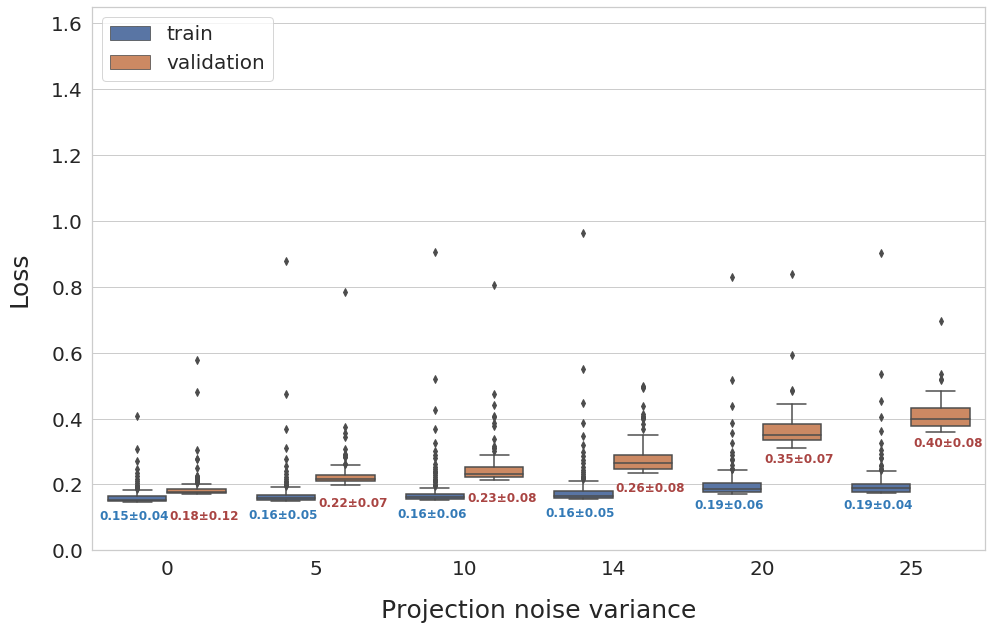
\includegraphics[height=8cm]{images/de_noises_nums.png}
        \caption{Variation of train and validation epoch losses w.r.t. noise levels in the projections of the asymmetric protein (5j0n).}
    \label{fig:distance-estimation-vary-projection-noise}
\end{figure}

\begin{figure}
    \centering
        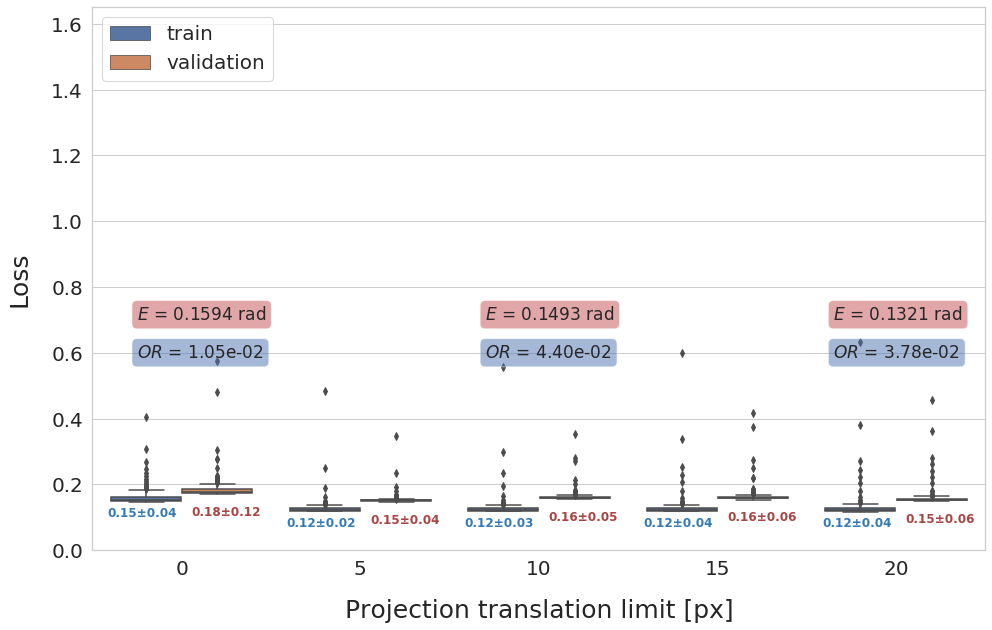
\includegraphics[height=8cm]{images/de_translation_nums.png}
        \caption{Variation of train and validation epoch losses w.r.t. projection translation of the asymmetric protein (5j0n).}
    \label{fig:distance-estimation-vary-projection-translation}
\end{figure}

\subsection{Orientation recovery from estimated distances}

\mdeff{Story: pipeline works but better distance estimation is needed for SOTA reconstruction.
Method is however promising because learned distance is robust to perturbations and recovery works if distance works.}

\begin{figure}
    \centering
    \begin{subfigure}[b]{0.45\textwidth}
        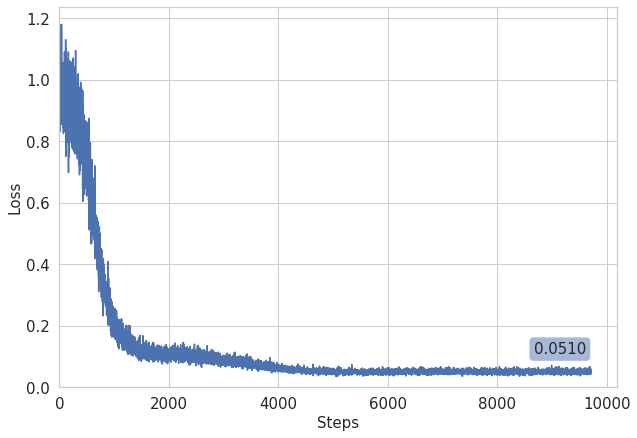
\includegraphics[height=5.5cm]{images/5j0n_noise0_angle_recovery.png}
        \caption{Noiseless projections}
    \end{subfigure}
    \hfill
    \begin{subfigure}[b]{0.5\textwidth}
    \centering
        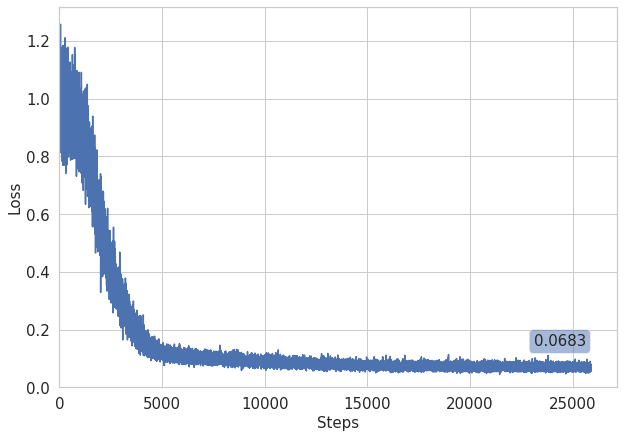
\includegraphics[height=5.5cm]{images/5j0n_noise16_angle_recovery.png}
        \caption{Noisy projections (variance 16)}
    \end{subfigure}
    \caption{ Orientation recovery loss of the asymmetric protein (5j0n).}
    \label{fig:orientation-recovery-loss}
\end{figure}

\begin{figure}
    \centering
    \begin{subfigure}[b]{0.45\textwidth}
        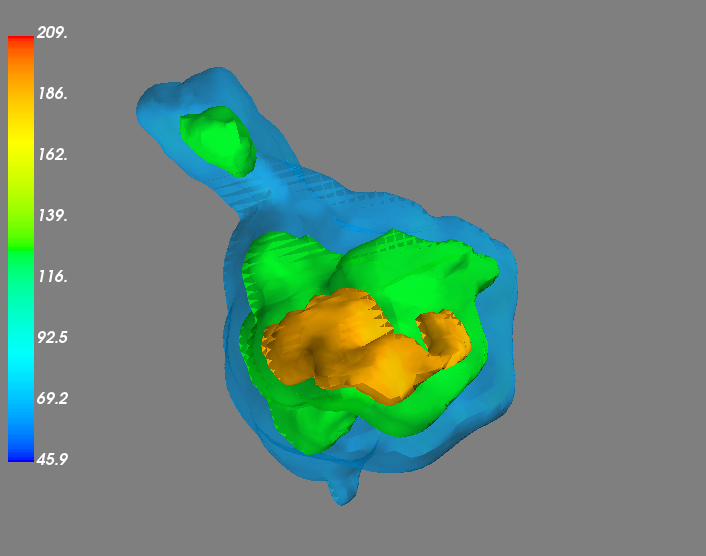
\includegraphics[height=5.5cm]{images/5j0n_reconstruction_GT.png}
        \caption{Ground truth}
    \end{subfigure}
    \hfill
    \begin{subfigure}[b]{0.5\textwidth}
    \centering
        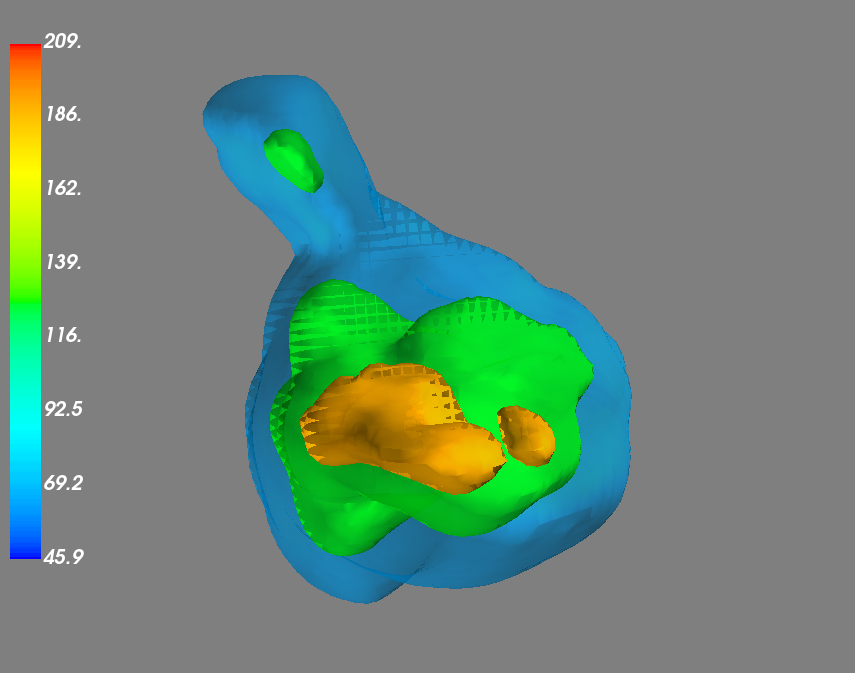
\includegraphics[height=5.5cm]{images/5j0n_reconstruction_noise0.png}
        \caption{Estimated}
    \end{subfigure}
    
    \caption{ Reconstruction of the asymmetric protein (5j0n).}
    \label{fig:reconstruction-noise0}
\end{figure}

\begin{figure}
    \centering
    \begin{subfigure}[b]{0.45\textwidth}
        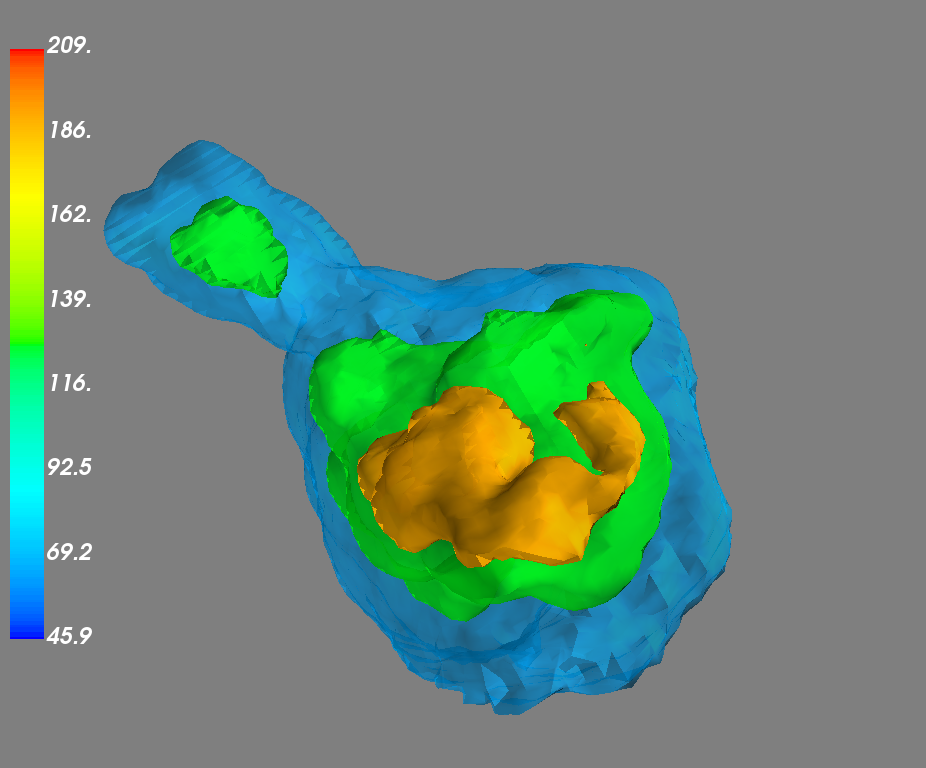
\includegraphics[height=5.5cm]{images/5j0n_reconstruction_GT_noise16.png}
        \caption{Ground truth}
    \end{subfigure}
    \hfill
    \begin{subfigure}[b]{0.5\textwidth}
    \centering
        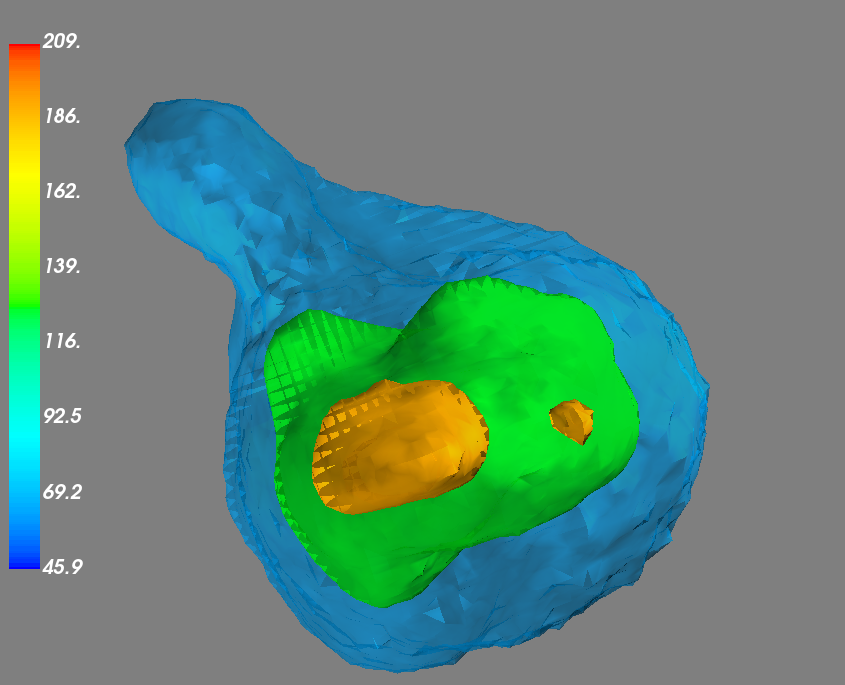
\includegraphics[height=5.5cm]{images/5j0n_reconstruction_noise16.png}
        \caption{Estimated}
    \end{subfigure}
    
    \caption{ Reconstruction of the asymmetric protein (5j0n) with noisy projections.}
    \label{fig:reconstruction-noise0}
\end{figure}

\todo{Justify threshold because of plateau (figref).
Show recovered orientations w.r.t.\ ground truth after alignment.}

\todo{Reconstruct the protein to show the full pipeline: from a set of projections to a reconstructed protein.
Emphasize that it's a naive reconstruction algorithm.}
